%% REPLACE sXXXXXXX with your student number
\def\studentNumber{s2617343}


%% START of YOUR ANSWERS
%% Add answers to the questions below, by replacing the text inside the brackets {} for \youranswer{ "Text to be replaced with your answer." }. 
%
% Do not delete the commands for adding figures and tables. Instead fill in the missing values with your experiment results, and replace the images with your own respective figures.
%
% You can generally delete the placeholder text, such as for example the text "Question Figure 3 - Replace the images ..." 
%
% There are 5 TEXT QUESTIONS. Replace the text inside the brackets of the command \youranswer with your answer to the question.
%
% There are also 3 "questions" to replace some placeholder FIGURES with your own, and 1 "question" asking you to fill in the missing entries in the TABLE provided. 
%
% NOTE! that questions are ordered by the order of appearance of their answers in the text, and not necessarily by the order you should tackle them. You should attempt to fill in the TABLE and FIGURES before discussing the results presented there. 
%
% NOTE! If for some reason you do not manage to produce results for some FIGURES and the TABLE, then you can get partial marks by discussing your expectations of the results in the relevant TEXT QUESTIONS. The TABLE specifically has enough information in it already for you to draw meaningful conclusions.
%
% Please refer to the coursework specification for more details.


%% - - - - - - - - - - - - TEXT QUESTIONS - - - - - - - - - - - - 

%% Question 1 - Use Figures 1, 2, and 3 to identify the Vanishing Gradient Problem (which of these model suffers from it, and what are the consequences depicted?).

% The average length for an answer to this question is approximately 1/5 of the columns in a 2-column page
\newcommand{\questionOne} {
\youranswer{By comparing Figure~\ref{fig:grad_flow_08} and Figure~\ref{fig:avg_grad_flow_38}, it is clear that VGG08 maintains significantly larger gradients across all layers (e.g., 0.025 at the bottom and 0.05-0.2 at the top). In contrast, VGG38 exhibits almost zero gradients beyond the bottom regression layer (~0.00035) and dimensionality reduction block (~0.000025), indicating a severe vanishing gradient problem.

This occurs because gradients diminish exponentially during backpropagation due to the chain rule, leaving top-layer gradients effectively zero. As a result, parameter updates fail in most layers, halting learning. This is reflected in Figure~\ref{fig:curves}, where VGG38's accuracy remains at 0 throughout training, despite increasing epochs.
}
}

%% Question 2 - Consider these results (including Figure 1 from \cite{he2016deep}). Discuss the relation between network capacity and overfitting, and whether, and how, this is reflected on these results. What other factors may have lead to this difference in performance?

% The average length for an answer to this question is
% approximately 1/5 of the columns in a 2-column page
\newcommand{\questionTwo} {
\youranswer{Generally, as network capacity increases, the model’s expressive power is expected to improve. However, larger-capacity models can suffer from overfitting, where the model learns data noise instead of general patterns. Additionally, differences in performance between networks of varying capacities may result from the vanishing gradient problem, as shown in Figure~\ref{fig:curves}. Larger models also introduce more parameters, requiring higher computational resources and leading to slower convergence.

In Figure 1 from \cite{he2016deep}, the 56-layer network underperforms compared to the 20-layer network, highlighting the model degradation problem. This issue is not necessarily due to overfitting but could stem from optimization challenges, such as insufficient convergence speed or difficulty propagating gradients effectively in deeper networks.}
}

%% Question 3 - In this coursework, we didn't incorporate residual connections to the downsampling layers. Explain and justify what would need to be changed in order to add residual connections to the downsampling layers. Give and explain 2 ways of incorporating these changes and discuss pros and cons of each.
\newcommand{\questionThree} {
\youranswer{Adding residual connections to a network requires that the input and output of the block have exactly the same shape; otherwise, additive residual connections cannot be performed. However, downsampling layers typically alter the output shape, making it incompatible with direct addition of residual connections.

We propose two solutions to address this issue. The first solution is to add a 1x1 convolution block to the residual connection to adjust the input shape, ensuring it matches the output shape. The advantage of this approach is its high flexibility, as the 1x1 convolution allows learning additional parameters to better retain input information. However, this method increases computational cost and model complexity.

The second solution is to add the same downsampling layer (e.g. average pooling) to the residual connection. This also aligns the input and output shapes, allowing residual addition. The advantage of this method is its simplicity and lack of additional computational overhead. However, the downside is that downsampling layers may lose important input information during the process.

Both methods enable residual connections in downsampling layers, but the choice depends on the specific requirements.}
}

%% Question 4 - Present and discuss the experiment results (all of the results and not just the ones you had to fill in) in Table 1 and Figures 4 and 5 (you may use any of the other Figures if you think they are relevant to your analysis). You will have to determine what data are relevant to the discussion, and what information can be extracted from it. Also, discuss what further experiments you would have ran on any combination of VGG08, VGG38, BN, RC in order to
% \begin{itemize}
%     \item Improve performance of the model trained (explain why you expect your suggested experiments will help with this).
%     \item Learn more about the behaviour of BN and RC (explain what you are trying to learn and how).
% \end{itemize}

% The average length for an answer to this question is approximately 1 of the columns in a 2-column page
\newcommand{\questionFour} {
\youranswer{From our experimental results, Batch Normalization (BN) and Residual Connections (RC) effectively alleviate the vanishing gradient problem and improve model performance. The specific effects can be observed in Table~\ref{tab:CIFAR_results}. First, by comparing VGG08 and VGG38, it is evident that deeper networks with larger capacity are more susceptible to the vanishing gradient problem. By adding BN and RC layers to VGG38, we observe a significant improvement in performance, as these methods successfully mitigate the gradient vanishing issue. Comparing the validation accuracy (val acc), we may infer that RC has a slightly greater impact than BN. 

Furthermore, by varying the learning rate, we found that the BN layer is less sensitive to learning rate changes, while the RC layer is more sensitive. This implies that adjusting the learning rate can further optimize networks with RC layers. Figure 6 from \cite{he2016deep} also demonstrates that BN effectively addresses gradient vanishing on its own, but the introduction of RC layers further enhances convergence on top of BN. Based on these experiments, we conclude that the best model configuration is VGG38 with BN and RC layers (learning rate of 1e-2). By analyzing its training curve (Figure~\ref{fig:training_curves_bestModel}) and gradient flow (Figure~\ref{fig:avg_grad_flow_bestModel}), we observe that this model mitigates the vanishing gradient problem well and achieves the highest validation accuracy of 59.92. However, there are signs of slight overfitting, and the validation curve exhibits greater volatility, possibly due to the model's sensitivity to the learning rate.

To further improve model performance, I suggest the following experimental designs:
1. Add BN and RC layers to VGG08 to test whether their benefits extend to shallower networks. Given their success with VGG38, this could reveal whether these methods are universally applicable or more effective in deeper networks.
2. Incorporate appropriate regularization methods, such as Dropout or L1 norm penalties, to mitigate the overfitting observed in the current best-performing model.

To further investigate the effects of BN and RC layers, I propose the following experimental directions:
1. Evaluate whether the effects of BN and RC remain consistent across networks of varying depths, such as VGG08 and VGG38.
2. Explore the effect of learning rates on networks with only RC layers, given our observation that learning rate has minimal impact on networks with only BN layers.
3. Examine whether BN and RC independently enhance model performance or if there is an interaction between the two methods that amplifies their effectiveness.

These additional experiments will provide deeper insights into the behavior and benefits of BN and RC layers across different set up.}
}


%% Question 5 - Briefly draw your conclusions based on the results from the previous sections (what are the take-away messages?) and conclude your report with a recommendation for future work. 

% Good recommendations for future work also draw on the broader literature (the papers already referenced are good starting points). Great recommendations for future work are not just incremental (an example of an incremental suggestion would be: ``we could also train with different learning rates'') but instead also identify meaningful questions or, in other words, questions with answers that might be somewhat more generally applicable. 

% For example, \citep{huang2017densely} end with \begin{quote}``Because of their compact internal representations and reduced feature redundancy, DenseNets may be good feature extractors for various computer vision tasks that build on convolutional features, e.g.,  [4,5].''\end{quote} 

% while \cite{bengio1993problem} state in their conclusions that \begin{quote}``There remains theoretical questions to be considered,  such as whether the problem with simple gradient descent  discussed in this paper would be observed with  chaotic attractors that are not  hyperbolic.''\\\end{quote}

% The length of this question description is indicative of the average length of a conclusion section
\newcommand{\questionFive} {
\youranswer{In this paper, we primarily investigated the vanishing gradient problem in deep networks. We found that simply increasing the number of layers in a model can lead to the gradient failing to propagate effectively to the upper layers, thereby hindering parameter updates. To address this issue, we explored two solutions: Batch Normalization (BN) and Residual Connections (RC). Both methods were applied to the original VGG38 model, and extensive experimental results demonstrated that these methods effectively mitigate the vanishing gradient problem. Additionally, our results highlight the potential for further experiments to explore the specific effects of BN and RC layers on model performance. 

Given that BN and RC layers have proven effective in addressing the vanishing gradient problem, we also observed that ResNet architectures fundamentally resolve the issue of network depth. By incorporating residual connections, ResNet enables deeper networks to maintain gradient flow. However, as noted in \cite{he2016deep}, the performance of very deep ResNets does not always surpass that of shallower ResNets. This suggests that network depth is no longer the primary limitation, and future research should instead focus on improving network optimization. Specifically, we recommend exploring methods to accelerate the convergence of large-capacity networks and address overfitting challenges.

In conclusion, while significant progress has been made in mitigating gradient-related issues, optimizing deeper networks remains an open problem. Future work could include designing better regularization techniques, exploring adaptive learning rate strategies for large-scale models, and investigating alternative architectures that balance depth, capacity, and generalization ability.}
}


%% - - - - - - - - - - - - FIGURES - - - - - - - - - - - - 

%% Question Figure 3 - Replace this image with a figure depicting the average gradient across layers, for the VGG38 model.

% \textit{(The provided figure is correct, and can be used in your analysis. It is partially obscured so you can get credit for producing your own copy).}
\newcommand{\questionFigureThree} {
\youranswer{
    Question Figure~\ref{fig:avg_grad_flow_38}
%
\begin{figure}[t]
    \centering
    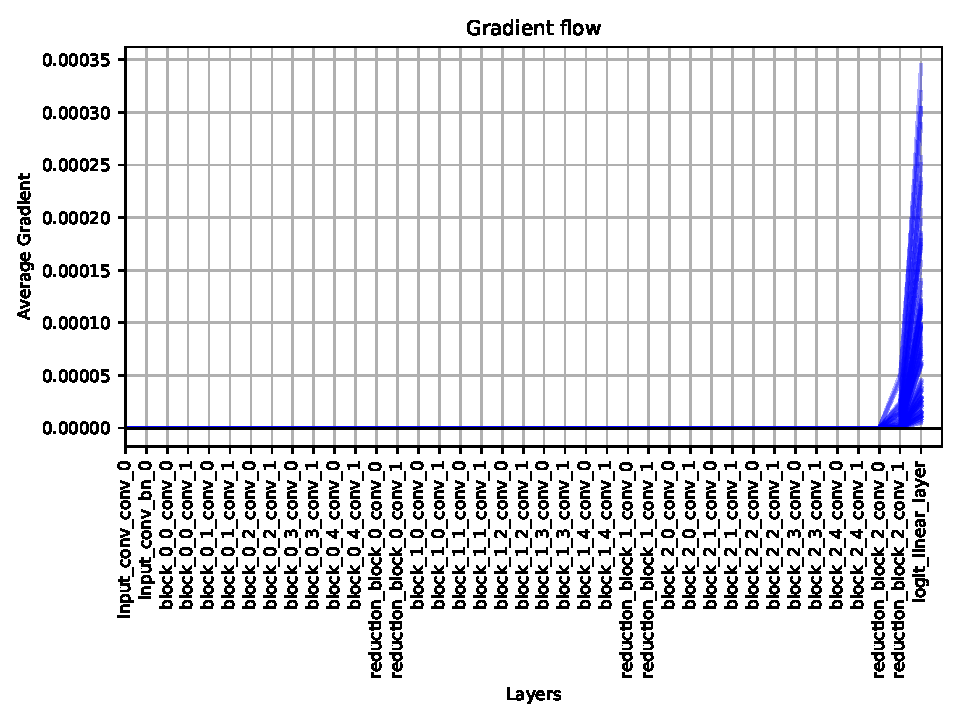
\includegraphics[width=\linewidth]{figures/myanswer_VGG_38.pdf} % figures/gradplot_38_watermarked.pdf
    \caption{Gradient Flow on VGG38}
    \label{fig:avg_grad_flow_38}
\end{figure}
}
}

%% Question Figure 4 - Replace this image with a figure depicting the training curves for the model with the best performance \textit{across experiments you have available (you don't need to run the experiments for the models we already give you results for)}. Edit the caption so that it clearly identifies the model and what is depicted.
\newcommand{\questionFigureFour} {
\youranswer{
    Question Figure~\ref{fig:training_curves_bestModel}
%
\begin{figure}[t]
    \centering
    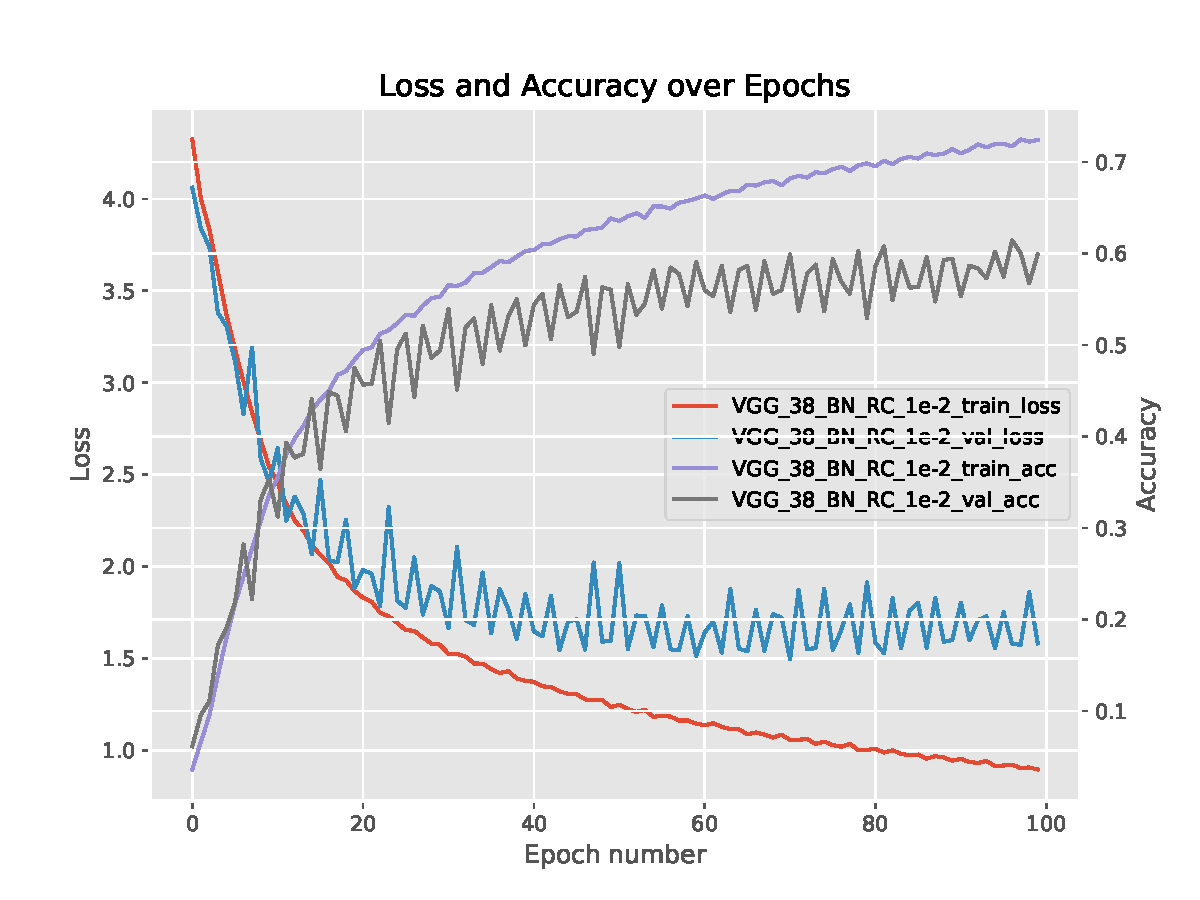
\includegraphics[width=\linewidth]{figures/myanswer_VGG_38_BN_RC_training_curve_big_figure.pdf}
    \caption{Training curves for VGG38 with Batch Normalisation and Residual Connection (Learning Rate 1e-2) in terms of cross-entropy error (left Y-axis) and classification accuracy (right Y-axis)}
    \label{fig:training_curves_bestModel}
\end{figure}
}
}

%% Question Figure 5 - Replace this image with a figure depicting the average gradient across layers, for the model with the best performance \textit{across experiments you have available (you don't need to run the experiments for the models we already give you results for)}. Edit the caption so that it clearly identifies the model and what is depicted.
\newcommand{\questionFigureFive} {
\youranswer{
    Question Figure~\ref{fig:avg_grad_flow_bestModel}
%
\begin{figure}[t]
    \centering
    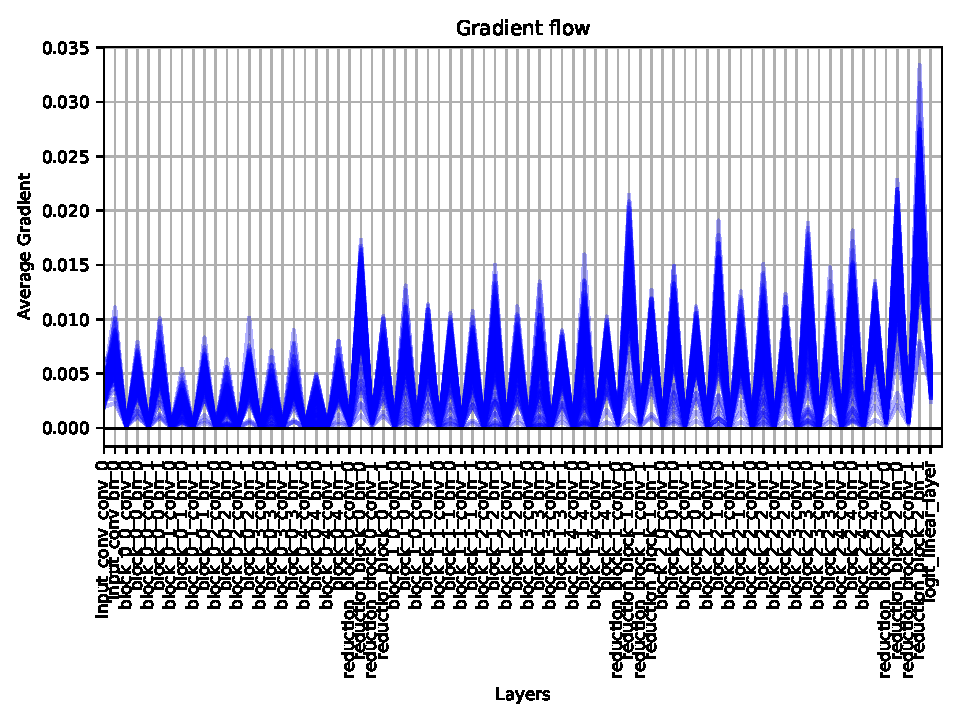
\includegraphics[width=\linewidth]{figures/myanswer_VGG_38_BN_RC_gradient_flow.pdf}
    \caption{Gradient Flow on VGG38 with Batch Normalisation and Residual Connection (Learning Rate 1e-2)}
    \label{fig:avg_grad_flow_bestModel}
\end{figure}
}
}

%% - - - - - - - - - - - - TABLES - - - - - - - - - - - - 

%% Question Table 1 - Fill in Table 1 with the results from your experiments on 
% \begin{enumerate}
%     \item \textit{VGG38 BN (LR 1e-3)}, and 
%     \item \textit{VGG38 BN + RC (LR 1e-2)}.
% \end{enumerate}
\newcommand{\questionTableOne} {
\youranswer{
    Question Table~\ref{tab:CIFAR_results}
%
\begin{table*}[t]
    \centering
    \begin{tabular}{lr|ccccc}
    \toprule
        Model                   & LR   & \# Params & Train loss & Train acc & Val loss & Val acc \\
    \midrule
        VGG08                   & 1e-3 & 60 K      &  1.74      & 51.59     & 1.95     & 46.84 \\
        VGG38                   & 1e-3 & 336 K     &  4.61      & 00.01     & 4.61     & 00.01 \\
        VGG38 BN                & 1e-3 & 339 K     &  1.70      & 52.16     & 1.84     & 48.08 \\
        VGG38 RC                & 1e-3 & 336 K     &  1.33      & 61.52     & 1.84     & 52.32 \\
        VGG38 BN + RC           & 1e-3 & 339 K     &  1.26      & 62.99     & 1.73     & 53.76 \\
        VGG38 BN                & 1e-2 & 339 K     &  1.70      & 52.28     & 1.99     & 46.72 \\
        VGG38 BN + RC           & 1e-2 & 339 K     &  0.90      & 72.43     & 1.58     & 59.92 \\
    \bottomrule
    \end{tabular}
    \caption{Experiment results (number of model parameters, Training and Validation loss and accuracy) for different combinations of VGG08, VGG38, Batch Normalisation (BN), and Residual Connections (RC), LR is learning rate.}
    \label{tab:CIFAR_results}
\end{table*} 
}
}

%% END of YOUR ANSWERS
